\documentclass[aspectratio=169]{beamer}
\usetheme{Bruno}

\title{Accompagner les agropasteurs de Diohine dans leur gouvernance du parc a Faidherbia Albida.}
\author{
    \vspace{-1em}
    L. Broutin$^{a,b,d}$, A. Fallot$^{a,b}$, A. Perrotton$^{c,d}$,\\
    A. Gonin$^{e}$, D. Masse$^{f}$, \textbf{E. Delay}$^{a,g}$
}
\institute{
    \vspace{-1.5em}
    $^{a}$ CIRAD, UMR SENS, F-34398 Montpellier, France

    $^{b}$ SENS, CIRAD, IRD, Université de Paul Valéry Montpellier 3, Montpellier, France. 

    $^{c}$ CIRAD, Forêts et Sociétés, F-34398 Montpellier, France.

    $^{d}$ Forêts et Sociétés, Univ Montpellier, CIRAD, Montpellier, France. 

    $^{e}$ Université Paris Nanterre, Laboratoire LAVUE, FR 

    $^{f}$ IRD, Eco\&Sols, Abidjan, Côte d’Ivoire

    $^{g}$ UMI UMMSCO,  Université Cheick Anta Diop, Dakar, Sénégal
}
\date{\today}
\background{background.jpeg}

\begin{document}

\maketitle

\begin{frame}{Zone d'étude}
    \begin{figure}
        \centering
        \includegraphics[width=10cm]{img/carte_localisation_diohine.png}
    \end{figure}
\end{frame}

\begin{frame}{Un travail ancré dans les aspirations locales}
    \begin{center}
        \vspace{-1em}
        \begin{figure}
            \centering
            \includegraphics[height = 4.5cm]{img/photoAspiration.png}~
            \includegraphics[height = 4.5cm]{img/modeleConceptuel.png}
            \caption{Aspirations ressorties de l’atelier du 07/05/2021, Perrotton et al 2021 }
        \end{figure}
    \end{center}
\end{frame}

\begin{frame}{Une urgence environnementale}
    \begin{center}
        \vspace{-1em}
        \begin{figure}
            \centering
            \includegraphics[height = 4.5cm]{img/desert.jpg}~
            \includegraphics[height = 6cm]{img/densiteArbres.png}
        \end{figure}
    \end{center}
\end{frame}

\begin{frame}{Problématique}
    \begin{center}
        \large{Par quelle gestion du parc agroforestier, pour faire face à la dégradation environnementale ?}
    \end{center}
\end{frame}

\begin{frame}{Un travail ancré dans les aspirations locales}
    \begin{center}
        \vspace{-1em}
        \begin{figure}
            \centering
            \includegraphics[height = 4.7cm]{img/emondage_faidherbia.png}~
            \includegraphics[height = 4.7cm]{img/atelierLucas.jpg}~
            \includegraphics[height = 4.7cm]{img/entretienChamp.jpg}
        \end{figure}
    \end{center}
\end{frame}

\begin{frame}{Le modèle  comme boussole}
    \begin{itemize}
        \item Qui guide la “démarche anthropologique” 
        \item Qui fait émerger des questionnements précis 
        \item Qui est fondé sur des données qualitatives provenant des entretiens et ateliers  
    \end{itemize}
    \begin{center}
        \vspace{-1em}
        \begin{figure}
            \centering
            \includegraphics[height = 5.7cm]{img/questionImplementation.png}
        \end{figure}
    \end{center}
\end{frame}

\begin{frame}{ComMod : un modèle intelligibile...}
    \begin{center}
        \vspace{-1em}
        \begin{figure}
            \centering
            \includegraphics[height = 6cm]{img/atelierPoster.jpg}~
            \includegraphics[height = 6cm]{img/poster2.png}
        \end{figure}
    \end{center}
\end{frame}

\begin{frame}{... mais un modèle quand même}
    \begin{center}
        \vspace{-1em}
        \begin{figure}
            \centering
            \includegraphics[height = 6cm]{img/ideModele.png}
        \end{figure}
    \end{center}
\end{frame}

\begin{frame}{Un modèle comme béquille pour le cerveau}
    \begin{center}
        \vspace{-1em}

        \begin{itemize}
            \item faire émerger des questionnements non-intuitifs,
            \item de fournir des supports de pensée (modèle actant)
        \end{itemize}
        \begin{figure}
            \centering
            \includegraphics[height = 5.5cm]{img/boxplotReunionDiscussion.png}~
            \includegraphics[height = 2cm]{img/OpenMOLE-Banner.png}
        \end{figure}
    \end{center}
\end{frame}

\begin{frame}{Questionner la viabilité !}
    \begin{figure}
        \centering
        \includegraphics[height = 6cm]{img/viabilité.png}~
        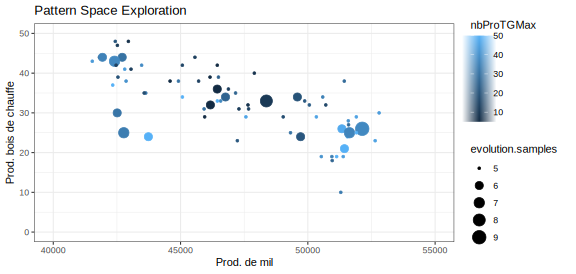
\includegraphics[height = 6cm]{../../../img/om_pse.png}
    \end{figure}
\end{frame}

\begin{frame}{Pour conclure ? }
    
\end{frame}

\end{document}
